\documentclass[oneside, a4paper,11pt]{book}
\usepackage[margin=1in]{geometry}

\usepackage{graphicx}
\usepackage[utf8]{inputenc} % allow utf-8 input
\usepackage[T1]{fontenc}    % use 8-bit T1 fonts
\usepackage{hyperref}       % hyperlinks
\usepackage{url}            % simple URL typesetting
\usepackage{booktabs}       % professional-quality tables
\usepackage{nicefrac}       % compact symbols for 1/2, etc.
\usepackage{microtype}      % microtypography

\usepackage{listings}
\usepackage{xcolor}
\definecolor{codegreen}{rgb}{0,0.6,0}
\definecolor{codegray}{rgb}{0.5,0.5,0.5}
\definecolor{codepurple}{rgb}{0.58,0,0.82}
\definecolor{backcolour}{rgb}{0.95,0.95,0.92}

\lstdefinestyle{mystyle}{
    backgroundcolor=\color{backcolour},
    commentstyle=\color{codegreen},
    keywordstyle=\color{magenta},
    numberstyle=\tiny\color{codegray},
    stringstyle=\color{codepurple},
    basicstyle=\ttfamily\footnotesize,
    breakatwhitespace=false,
    breaklines=true,
    captionpos=b,
    keepspaces=true,
    numbers=left,
    numbersep=5pt,
    showspaces=false,
    showstringspaces=false,
    showtabs=false,
    tabsize=2
}
\lstset{style=mystyle}


\usepackage[autostyle]{csquotes}
\usepackage{dsfont}

%\usepackage{algorithm,algpseudocode}
\usepackage[ruled,vlined]{algorithm2e}
\usepackage{multicol}

\usepackage{hyperref}
\usepackage{amssymb}

\setlength{\parindent}{0pt}
\setlength{\parskip}{1em}

\newtheorem{theorem}{Theorem}
\newtheorem{definition}{Definition}
\newtheorem{proposition}{Proposition}
\newtheorem{corollary}{Corollary}

\newcommand\scalemath[2]{\scalebox{#1}{\mbox{\ensuremath{\displaystyle #2}}}}

\newcommand{\red}[1]{\textcolor{red}{#1}}
\newcommand{\blue}[1]{\textcolor{blue}{#1}}
\newcommand{\magenta}[1]{\textcolor{magenta}{#1}}
\newcommand{\green}[1]{\textcolor{green}{#1}}
\newcommand{\cyan}[1]{\textcolor{cyan}{#1}}

%%%%% NEW MATH DEFINITIONS %%%%%
\usepackage{amsmath,amsfonts,bm}
\usepackage{xspace}
\usepackage[nameinlink]{cleveref}


\crefformat{section}{\S#2#1#3} % see manual of cleveref, section 8.2.1
\crefname{algorithm}{Alg.}{Algs.}
\crefformat{subsection}{\S#2#1#3}
\Crefname{equation}{Eq.}{Eqs.}
\Crefname{figure}{Fig.}{Figs.}

%% abbr 
\newcommand{\ie}{{\em i.e.,}\xspace}
\newcommand{\cf}{{\em c.f.,}\xspace}
\newcommand{\eg}{{\em e.g.,}\xspace}
\newcommand{\etal}{{\em et al.,}\xspace}
\newcommand{\wrt}{\emph{w.r.t.}\xspace}
\newcommand{\aka}{\emph{a.k.a.}\xspace}
\newcommand{\resp}{\emph{resp.}\xspace}


\newcommand{\pos}{${pos}$}


%%% inline lists
\newcommand{\Ni}{({\em i})~}
\newcommand{\Nii}{({\em ii})~}
\newcommand{\Niii}{({\em iii})~}
\newcommand{\Niv}{({\em iv})~}
\newcommand{\Nv}{({\em v})~}
\newcommand{\Na}{({\em a})~}
\newcommand{\Nb}{({\em b})~}
\newcommand{\Nc}{({\em c})~}
\newcommand{\Nd}{({\em d})~}
\newcommand{\Ne}{({\em e})~}
\newcommand{\Nf}{({\em f})~}


\newcommand{\comm}[1]{\textcolor{blue}{\noindent #1}}
\newcommand{\alert}[1]{\textcolor{red}{\noindent$\Rightarrow$ #1}}
\newcommand{\red}[1]{\textcolor{red}{#1}}
\newcommand{\blue}[1]{\textcolor{blue}{#1}}
\newcommand{\magenta}[1]{\textcolor{magenta}{#1}}
\newcommand{\green}[1]{\textcolor{green}{#1}}
\newcommand{\teal}[1]{\textcolor{teal}{#1}}
\newcommand{\add}[1]{\textcolor{black}{#1}}

%\usepackage{amsmath,amsfonts,bm}
%\usepackage[tbtags]{amsmath}

% Mark sections of captions for referring to divisions of figures
\newcommand{\figleft}{{\em (Left)}}
\newcommand{\figcenter}{{\em (Center)}}
\newcommand{\figright}{{\em (Right)}}
\newcommand{\figtop}{{\em (Top)}}
\newcommand{\figbottom}{{\em (Bottom)}}
\newcommand{\captiona}{{\em (a)}}
\newcommand{\captionb}{{\em (b)}}
\newcommand{\captionc}{{\em (c)}}
\newcommand{\captiond}{{\em (d)}}


\newtheorem{prop}{Proposition}

\newcommand{\sarrow}[1][4pt]{\!\mathrel{%
   \vcenter{\hbox{\rule[-.5\fontdimen8\textfont3]{#1}{\fontdimen8\textfont3}}}%
   \mkern-4mu\hbox{\usefont{U}{lasy}{m}{n}\symbol{41}}}\!}
\makeatletter   
\newcommand{\sveryshortarrow}[1][3pt]{\mathrel{%
    \vcenter{\hbox{\rule[-.5\fontdimen8\scriptfont3]
               {\scriptratio\dimexpr#1\relax}{\fontdimen8\scriptfont3}}}%
   \mkern-4mu\hbox{\let\f@size\sf@size\usefont{U}{lasy}{m}{n}\symbol{41}}}}
\makeatother

% \newcommand{\sarrow}{{\veryshortarrow}}

\newtheorem{defi}{Definition}

% Highlight a newly defined term
\newcommand{\newterm}[1]{{\bf #1}}


% Figure reference, lower-case.
\def\figref#1{figure~\ref{#1}}
% Figure reference, capital. For start of sentence
\def\Figref#1{Figure~\ref{#1}}
\def\twofigref#1#2{figures \ref{#1} and \ref{#2}}
\def\quadfigref#1#2#3#4{figures \ref{#1}, \ref{#2}, \ref{#3} and \ref{#4}}
% Section reference, lower-case.
\def\secref#1{section~\ref{#1}}
% Section reference, capital.
\def\Secref#1{Section~\ref{#1}}
% Reference to two sections.
\def\twosecrefs#1#2{sections \ref{#1} and \ref{#2}}
% Reference to three sections.
\def\secrefs#1#2#3{sections \ref{#1}, \ref{#2} and \ref{#3}}
% Reference to an equation, lower-case.
\def\eqref#1{equation~\ref{#1}}
% Reference to an equation, upper case
\def\Eqref#1{Equation~\ref{#1}}
% A raw reference to an equation---avoid using if possible
\def\plaineqref#1{\ref{#1}}
% Reference to a chapter, lower-case.
\def\chapref#1{chapter~\ref{#1}}
% Reference to an equation, upper case.
\def\Chapref#1{Chapter~\ref{#1}}
% Reference to a range of chapters
\def\rangechapref#1#2{chapters\ref{#1}--\ref{#2}}
% Reference to an algorithm, lower-case.
\def\algref#1{algorithm~\ref{#1}}
% Reference to an algorithm, upper case.
\def\Algref#1{Algorithm~\ref{#1}}
\def\twoalgref#1#2{algorithms \ref{#1} and \ref{#2}}
\def\Twoalgref#1#2{Algorithms \ref{#1} and \ref{#2}}
% Reference to a part, lower case
\def\partref#1{part~\ref{#1}}
% Reference to a part, upper case
\def\Partref#1{Part~\ref{#1}}
\def\twopartref#1#2{parts \ref{#1} and \ref{#2}}

\def\ceil#1{\lceil #1 \rceil}
\def\floor#1{\lfloor #1 \rfloor}
\def\1{\bm{1}}
\newcommand{\train}{\mathcal{D}}
\newcommand{\valid}{\mathcal{D_{\mathrm{valid}}}}
\newcommand{\test}{\mathcal{D_{\mathrm{test}}}}

\def\eps{{\epsilon}}


% Random variables
\def\reta{{\textnormal{$\eta$}}}
\def\ra{{\textnormal{a}}}
\def\rb{{\textnormal{b}}}
\def\rc{{\textnormal{c}}}
\def\rd{{\textnormal{d}}}
\def\re{{\textnormal{e}}}
\def\rf{{\textnormal{f}}}
\def\rg{{\textnormal{g}}}
\def\rh{{\textnormal{h}}}
\def\ri{{\textnormal{i}}}
\def\rj{{\textnormal{j}}}
\def\rk{{\textnormal{k}}}
\def\rl{{\textnormal{l}}}
% rm is already a command, just don't name any random variables m
\def\rn{{\textnormal{n}}}
\def\ro{{\textnormal{o}}}
\def\rp{{\textnormal{p}}}
\def\rq{{\textnormal{q}}}
\def\rr{{\textnormal{r}}}
\def\rs{{\textnormal{s}}}
\def\rt{{\textnormal{t}}}
\def\ru{{\textnormal{u}}}
\def\rv{{\textnormal{v}}}
\def\rw{{\textnormal{w}}}
\def\rx{{\textnormal{x}}}
\def\ry{{\textnormal{y}}}
\def\rz{{\textnormal{z}}}

% Random vectors
\def\rvepsilon{{\mathbf{\epsilon}}}
\def\rvtheta{{\mathbf{\theta}}}
\def\rva{{\mathbf{a}}}
\def\rvb{{\mathbf{b}}}
\def\rvc{{\mathbf{c}}}
\def\rvd{{\mathbf{d}}}
\def\rve{{\mathbf{e}}}
\def\rvf{{\mathbf{f}}}
\def\rvg{{\mathbf{g}}}
\def\rvh{{\mathbf{h}}}
\def\rvu{{\mathbf{i}}}
\def\rvj{{\mathbf{j}}}
\def\rvk{{\mathbf{k}}}
\def\rvl{{\mathbf{l}}}
\def\rvm{{\mathbf{m}}}
\def\rvn{{\mathbf{n}}}
\def\rvo{{\mathbf{o}}}
\def\rvp{{\mathbf{p}}}
\def\rvq{{\mathbf{q}}}
\def\rvr{{\mathbf{r}}}
\def\rvs{{\mathbf{s}}}
\def\rvt{{\mathbf{t}}}
\def\rvu{{\mathbf{u}}}
\def\rvv{{\mathbf{v}}}
\def\rvw{{\mathbf{w}}}
\def\rvx{{\mathbf{x}}}
\def\rvy{{\mathbf{y}}}
\def\rvz{{\mathbf{z}}}

% Elements of random vectors
\def\erva{{\textnormal{a}}}
\def\ervb{{\textnormal{b}}}
\def\ervc{{\textnormal{c}}}
\def\ervd{{\textnormal{d}}}
\def\erve{{\textnormal{e}}}
\def\ervf{{\textnormal{f}}}
\def\ervg{{\textnormal{g}}}
\def\ervh{{\textnormal{h}}}
\def\ervi{{\textnormal{i}}}
\def\ervj{{\textnormal{j}}}
\def\ervk{{\textnormal{k}}}
\def\ervl{{\textnormal{l}}}
\def\ervm{{\textnormal{m}}}
\def\ervn{{\textnormal{n}}}
\def\ervo{{\textnormal{o}}}
\def\ervp{{\textnormal{p}}}
\def\ervq{{\textnormal{q}}}
\def\ervr{{\textnormal{r}}}
\def\ervs{{\textnormal{s}}}
\def\ervt{{\textnormal{t}}}
\def\ervu{{\textnormal{u}}}
\def\ervv{{\textnormal{v}}}
\def\ervw{{\textnormal{w}}}
\def\ervx{{\textnormal{x}}}
\def\ervy{{\textnormal{y}}}
\def\ervz{{\textnormal{z}}}

% Random matrices
\def\rmA{{\mathbf{A}}}
\def\rmB{{\mathbf{B}}}
\def\rmC{{\mathbf{C}}}
\def\rmD{{\mathbf{D}}}
\def\rmE{{\mathbf{E}}}
\def\rmF{{\mathbf{F}}}
\def\rmG{{\mathbf{G}}}
\def\rmH{{\mathbf{H}}}
\def\rmI{{\mathbf{I}}}
\def\rmJ{{\mathbf{J}}}
\def\rmK{{\mathbf{K}}}
\def\rmL{{\mathbf{L}}}
\def\rmM{{\mathbf{M}}}
\def\rmN{{\mathbf{N}}}
\def\rmO{{\mathbf{O}}}
\def\rmP{{\mathbf{P}}}
\def\rmQ{{\mathbf{Q}}}
\def\rmR{{\mathbf{R}}}
\def\rmS{{\mathbf{S}}}
\def\rmT{{\mathbf{T}}}
\def\rmU{{\mathbf{U}}}
\def\rmV{{\mathbf{V}}}
\def\rmW{{\mathbf{W}}}
\def\rmX{{\mathbf{X}}}
\def\rmY{{\mathbf{Y}}}
\def\rmZ{{\mathbf{Z}}}

% Elements of random matrices
\def\ermA{{\textnormal{A}}}
\def\ermB{{\textnormal{B}}}
\def\ermC{{\textnormal{C}}}
\def\ermD{{\textnormal{D}}}
\def\ermE{{\textnormal{E}}}
\def\ermF{{\textnormal{F}}}
\def\ermG{{\textnormal{G}}}
\def\ermH{{\textnormal{H}}}
\def\ermI{{\textnormal{I}}}
\def\ermJ{{\textnormal{J}}}
\def\ermK{{\textnormal{K}}}
\def\ermL{{\textnormal{L}}}
\def\ermM{{\textnormal{M}}}
\def\ermN{{\textnormal{N}}}
\def\ermO{{\textnormal{O}}}
\def\ermP{{\textnormal{P}}}
\def\ermQ{{\textnormal{Q}}}
\def\ermR{{\textnormal{R}}}
\def\ermS{{\textnormal{S}}}
\def\ermT{{\textnormal{T}}}
\def\ermU{{\textnormal{U}}}
\def\ermV{{\textnormal{V}}}
\def\ermW{{\textnormal{W}}}
\def\ermX{{\textnormal{X}}}
\def\ermY{{\textnormal{Y}}}
\def\ermZ{{\textnormal{Z}}}

% Vectors
\def\vzero{{\bm{0}}}
\def\vone{{\bm{1}}}
\def\vmu{{\bm{\mu}}}
\def\vtheta{{\bm{\theta}}}
\def\va{{\bm{a}}}
\def\vb{{\bm{b}}}
\def\vc{{\bm{c}}}
\def\vd{{\bm{d}}}
\def\ve{{\bm{e}}}
\def\vf{{\bm{f}}}
\def\vg{{\bm{g}}}
\def\vh{{\bm{h}}}
\def\vi{{\bm{i}}}
\def\vj{{\bm{j}}}
\def\vk{{\bm{k}}}
\def\vl{{\bm{l}}}
\def\vm{{\bm{m}}}
\def\vn{{\bm{n}}}
\def\vo{{\bm{o}}}
\def\vp{{\bm{p}}}
\def\vq{{\bm{q}}}
\def\vr{{\bm{r}}}
\def\vs{{\bm{s}}}
\def\vt{{\bm{t}}}
\def\vu{{\bm{u}}}
\def\vv{{\bm{v}}}
\def\vw{{\bm{w}}}
\def\vx{{\bm{x}}}
\def\vy{{\bm{y}}}
\def\vz{{\bm{z}}}

\def\vip{{\bm{i}\bm{p}}}

\def\vdelta{{\bm{\delta}}}
\def\valphaa{{\bm{\alpha}}}

% Elements of vectors
\def\evalpha{{\alpha}}
\def\evbeta{{\beta}}
\def\evepsilon{{\epsilon}}
\def\evlambda{{\lambda}}
\def\evomega{{\omega}}
\def\evmu{{\mu}}
\def\evpsi{{\psi}}
\def\evsigma{{\sigma}}
\def\evtheta{{\theta}}
\def\eva{{a}}
\def\evb{{b}}
\def\evc{{c}}
\def\evd{{d}}
\def\eve{{e}}
\def\evf{{f}}
\def\evg{{g}}
\def\evh{{h}}
\def\evi{{i}}
\def\evj{{j}}
\def\evk{{k}}
\def\evl{{l}}
\def\evm{{m}}
\def\evn{{n}}
\def\evo{{o}}
\def\evp{{p}}
\def\evq{{q}}
\def\evr{{r}}
\def\evs{{s}}
\def\evt{{t}}
\def\evu{{u}}
\def\evv{{v}}
\def\evw{{w}}
\def\evx{{x}}
\def\evy{{y}}
\def\evz{{z}}

% Matrix
\def\m1{{\bm{1}}}
\def\mA{{\bm{A}}}
\def\mB{{\bm{B}}}
\def\mC{{\bm{C}}}
\def\mD{{\bm{D}}}
\def\mE{{\bm{E}}}
\def\mF{{\bm{F}}}
\def\mG{{\bm{G}}}
\def\mH{{\bm{H}}}
\def\mI{{\bm{I}}}
\def\mJ{{\bm{J}}}
\def\mK{{\bm{K}}}
\def\mL{{\bm{L}}}
\def\mM{{\bm{M}}}
\def\mN{{\bm{N}}}
\def\mO{{\bm{O}}}
\def\mP{{\bm{P}}}
\def\mQ{{\bm{Q}}}
\def\mR{{\bm{R}}}
\def\mS{{\bm{S}}}
\def\mT{{\bm{T}}}
\def\mU{{\bm{U}}}
\def\mV{{\bm{V}}}
\def\mW{{\bm{W}}}
\def\mX{{\bm{X}}}
\def\mY{{\bm{Y}}}
\def\mZ{{\bm{Z}}}
\def\mBeta{{\bm{\beta}}}
\def\mPhi{{\bm{\Phi}}}
\def\mLambda{{\bm{\Lambda}}}
\def\mSigma{{\bm{\Sigma}}}

% Tensor
\DeclareMathAlphabet{\mathsfit}{\encodingdefault}{\sfdefault}{m}{sl}
\SetMathAlphabet{\mathsfit}{bold}{\encodingdefault}{\sfdefault}{bx}{n}

\newcommand{\tens}[1]{\bm{\mathsfit{#1}}}


\def\tA{{\tens{A}}}
\def\tB{{\tens{B}}}
\def\tC{{\tens{C}}}
\def\tD{{\tens{D}}}
\def\tE{{\tens{E}}}
\def\tF{{\tens{F}}}
\def\tG{{\tens{G}}}
\def\tH{{\tens{H}}}
\def\tI{{\tens{I}}}
\def\tJ{{\tens{J}}}
\def\tK{{\tens{K}}}
\def\tL{{\tens{L}}}
\def\tM{{\tens{M}}}
\def\tN{{\tens{N}}}
\def\tO{{\tens{O}}}
\def\tP{{\tens{P}}}
\def\tQ{{\tens{Q}}}
\def\tR{{\tens{R}}}
\def\tS{{\tens{S}}}
\def\tT{{\tens{T}}}
\def\tU{{\tens{U}}}
\def\tV{{\tens{V}}}
\def\tW{{\tens{W}}}
\def\tX{{\tens{X}}}
\def\tY{{\tens{Y}}}
\def\tZ{{\tens{Z}}}


% Graph
\def\gA{{\mathcal{A}}}
\def\gB{{\mathcal{B}}}
\def\gC{{\mathcal{C}}}
\def\gD{{\mathcal{D}}}
\def\gE{{\mathcal{E}}}
\def\gF{{\mathcal{F}}}
\def\gG{{\mathcal{G}}}
\def\gH{{\mathcal{H}}}
\def\gI{{\mathcal{I}}}
\def\gJ{{\mathcal{J}}}
\def\gK{{\mathcal{K}}}
\def\gL{{\mathcal{L}}}
\def\gM{{\mathcal{M}}}
\def\gN{{\mathcal{N}}}
\def\gO{{\mathcal{O}}}
\def\gP{{\mathcal{P}}}
\def\gQ{{\mathcal{Q}}}
\def\gR{{\mathcal{R}}}
\def\gS{{\mathcal{S}}}
\def\gT{{\mathcal{T}}}
\def\gU{{\mathcal{U}}}
\def\gV{{\mathcal{V}}}
\def\gW{{\mathcal{W}}}
\def\gX{{\mathcal{X}}}
\def\gY{{\mathcal{Y}}}
\def\gZ{{\mathcal{Z}}}
\def\gSP{{\mathcal{S}\mathcal{P}}}
\def\gLS{{\mathcal{L}\mathcal{S}}}
\def\gLU{{\mathcal{L}\mathcal{U}}}
\def\gST{{\mathcal{S}\mathcal{T}}}

% Sets
\def\sA{{\mathbb{A}}}
\def\sB{{\mathbb{B}}}
\def\sC{{\mathbb{C}}}
\def\sD{{\mathbb{D}}}
% Don't use a set called E, because this would be the same as our symbol
% for expectation.
\def\sF{{\mathbb{F}}}
\def\sG{{\mathbb{G}}}
\def\sH{{\mathbb{H}}}
\def\sI{{\mathbb{I}}}
\def\sJ{{\mathbb{J}}}
\def\sK{{\mathbb{K}}}
\def\sL{{\mathbb{L}}}
\def\sM{{\mathbb{M}}}
\def\sN{{\mathbb{N}}}
\def\sO{{\mathbb{O}}}
\def\sP{{\mathbb{P}}}
\def\sQ{{\mathbb{Q}}}
\def\sR{{\mathbb{R}}}
\def\sS{{\mathbb{S}}}
\def\sT{{\mathbb{T}}}
\def\sU{{\mathbb{U}}}
\def\sV{{\mathbb{V}}}
\def\sW{{\mathbb{W}}}
\def\sX{{\mathbb{X}}}
\def\sY{{\mathbb{Y}}}
\def\sZ{{\mathbb{Z}}}

\def\sSB{{\mathbb{S}\mathbb{B}}}

% Entries of a matrix
\def\emLambda{{\Lambda}}
\def\emA{{A}}
\def\emB{{B}}
\def\emC{{C}}
\def\emD{{D}}
\def\emE{{E}}
\def\emF{{F}}
\def\emG{{G}}
\def\emH{{H}}
\def\emI{{I}}
\def\emJ{{J}}
\def\emK{{K}}
\def\emL{{L}}
\def\emM{{M}}
\def\emN{{N}}
\def\emO{{O}}
\def\emP{{P}}
\def\emQ{{Q}}
\def\emR{{R}}
\def\emS{{S}}
\def\emT{{T}}
\def\emU{{U}}
\def\emV{{V}}
\def\emW{{W}}
\def\emX{{X}}
\def\emY{{Y}}
\def\emZ{{Z}}
\def\emSigma{{\Sigma}}

% entries of a tensor
% Same font as tensor, without \bm wrapper
\newcommand{\etens}[1]{\mathsfit{#1}}
\def\etLambda{{\etens{\Lambda}}}
\def\etA{{\etens{A}}}
\def\etB{{\etens{B}}}
\def\etC{{\etens{C}}}
\def\etD{{\etens{D}}}
\def\etE{{\etens{E}}}
\def\etF{{\etens{F}}}
\def\etG{{\etens{G}}}
\def\etH{{\etens{H}}}
\def\etI{{\etens{I}}}
\def\etJ{{\etens{J}}}
\def\etK{{\etens{K}}}
\def\etL{{\etens{L}}}
\def\etM{{\etens{M}}}
\def\etN{{\etens{N}}}
\def\etO{{\etens{O}}}
\def\etP{{\etens{P}}}
\def\etQ{{\etens{Q}}}
\def\etR{{\etens{R}}}
\def\etS{{\etens{S}}}
\def\etT{{\etens{T}}}
\def\etU{{\etens{U}}}
\def\etV{{\etens{V}}}
\def\etW{{\etens{W}}}
\def\etX{{\etens{X}}}
\def\etY{{\etens{Y}}}
\def\etZ{{\etens{Z}}}

% The true underlying data generating distribution
\newcommand{\pdata}{p_{\rm{data}}}
% The empirical distribution defined by the training set
\newcommand{\ptrain}{\hat{p}_{\rm{data}}}
\newcommand{\Ptrain}{\hat{P}_{\rm{data}}}
% The model distribution
\newcommand{\pmodel}{p_{\rm{model}}}
\newcommand{\Pmodel}{P_{\rm{model}}}
\newcommand{\ptildemodel}{\tilde{p}_{\rm{model}}}
% Stochastic autoencoder distributions
\newcommand{\pencode}{p_{\rm{encoder}}}
\newcommand{\pdecode}{p_{\rm{decoder}}}
\newcommand{\precons}{p_{\rm{reconstruct}}}

\newcommand{\laplace}{\mathrm{Laplace}} % Laplace distribution

\newcommand{\E}{\mathbb{E}}
\newcommand{\Ls}{\mathcal{L}}
\newcommand{\R}{\mathbb{R}}
\newcommand{\emp}{\tilde{p}}
\newcommand{\lr}{\alpha}
\newcommand{\reg}{\lambda}
\newcommand{\rect}{\mathrm{rectifier}}
\newcommand{\softmax}{\mathrm{softmax}}
%\newcommand{\softmax}{\mathcal{S}}


\newcommand{\ptr}{\rho}
\newcommand{\bptr}{bp}
\newcommand{\sptr}{sp}
\newcommand{\gptr}{gp}
%\newcommand{\lc}{lc}
\newcommand{\blb}{uc}
\newcommand{\glb}{gc}



\newcommand{\sigmoid}{\sigma}
\newcommand{\softplus}{\zeta}
\newcommand{\KL}{D_{\mathrm{KL}}}
\newcommand{\Var}{\mathrm{Var}}
\newcommand{\standarderror}{\mathrm{SE}}
\newcommand{\Cov}{\mathrm{Cov}}
% Wolfram Mathworld says $L^2$ is for function spaces and $\ell^2$ is for vectors
% But then they seem to use $L^2$ for vectors throughout the site, and so does
% wikipedia.
\newcommand{\normlzero}{L^0}
\newcommand{\normlone}{L^1}
\newcommand{\normltwo}{L^2}
\newcommand{\normlp}{L^p}
\newcommand{\normmax}{L^\infty}

\newcommand{\parents}{Pa} % See usage in notation.tex. Chosen to match Daphne's book.

\DeclareMathOperator*{\argmax}{\operatorname{argmax}}
\DeclareMathOperator*{\argmin}{\operatorname{argmin}}
\DeclareMathOperator*{\sup}{\operatorname{sup}}

\DeclareMathOperator{\sign}{sign}
\DeclareMathOperator{\Tr}{Tr}
\DeclareMathOperator{\real}{\rm I\!R}
\DeclareMathOperator*{\pop}{pop}
\DeclareMathOperator*{\push}{push}
\let\ab\allowbreak
% add specicial symbols
\def\blackcheck{\tikz\fill[scale=0.4, color=black](0,.35) -- (.25,0) -- (1,.7) -- (.25,.15) -- cycle;}


\begin{document}

\author{%
	Han Cheol Moon\\
	School of Computer Science and Engineering\\
	Nanyang Technological University\\
	Singapore\\
	\texttt{hancheol001@edu.ntu.edu.sg}
}
\title{Latent Variable Models}
\date{\today}

\frontmatter
\maketitle
\tableofcontents
\newpage

\mainmatter
\chapter{Introduction}
\section{Introduction}
\subsection{Motivation of Latent Variable Models}
\label{sec:intro_motivation}
If we knew a corresponding latent variable for each observation, then modelling might be easier. Imagine, how can we find $z^* = \argmaxE_{z} p(\mathbf{x|z})$ for the data $\mathbf{x}$ as shown in Fig. \ref{fig:clusters}(b)

\begin{figure}[h]
	\begin{center}			
		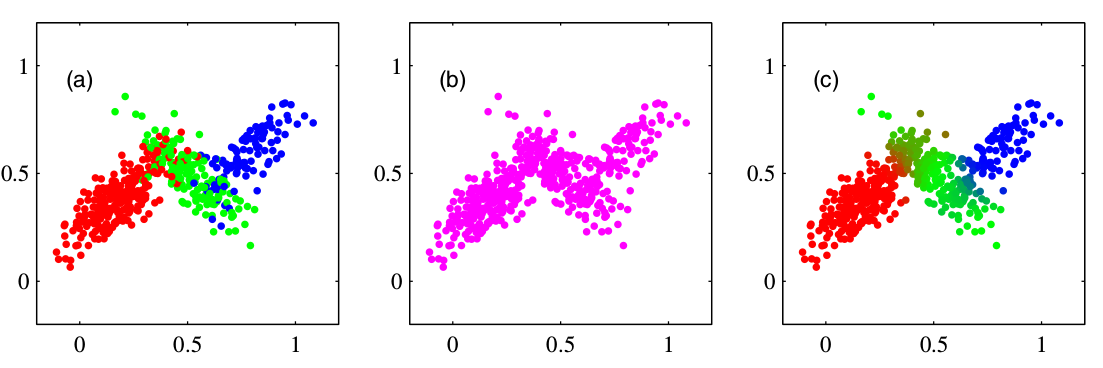
\includegraphics[scale=0.25]{./images/latent.png}
	\end{center}
	\caption{(a) Complete data set $p(\mathbf{x|z})$. (b) Incomplete data set $p(\mathbf{x})$. (c) Inference result}
	\label{fig:clusters}
\end{figure}
For example, we want to model the complete data set $p(\mathbf{x|z})$ under the i.i.d. assumption 
\begin{equation*}
p(\mathbf{x}_i, \mathbf{z}_i|\boldsymbol{\theta}) = 
\begin{cases}
p(\mathcal{C}_1)p(\mathbf{x}_i|\mathcal{C}_1) \textrm{ if } z_i=0\\
p(\mathcal{C}_2)p(\mathbf{x}_i|\mathcal{C}_2) \textrm{ if } z_i=1\\
p(\mathcal{C}_3)p(\mathbf{x}_i|\mathcal{C}_3) \textrm{ if } z_i=2\\
\end{cases}
\end{equation*}
\begin{align*}
p(\mathbf{x}_1, \mathbf{x}_2,...,\mathbf{x}_N, \mathbf{z}_1, \mathbf{z}_2, ..., \mathbf{z}_N|\boldsymbol{\theta}) = \prod_{n=1}^{N}\prod_{k=1}^{K}\pi_k^{z_{nk}}\mathcal{N}(\mathbf{x}_n|\boldsymbol{\mu}_k, \boldsymbol{\Sigma}_k)^{z_{nk}}
\end{align*}
, where $\pi_k=p(\mathcal{C}_k)$ and $p(\mathbf{x}_i|\mathcal{C}_k)=\mathcal{N}(\mathbf{x}_n|\boldsymbol{\mu}_k, \boldsymbol{\Sigma}_k)$. However, in many cases, it is not observable. 

%In this case, what we can only do is find a posterior $p(\mathbf{x}|\mathbf{z},\boldsymbol{\theta})$.



\section{K-Means Clustering}
Suppose we have a data set $\mathbf{X} = \{\mathbf{x}_1,...,\mathbf{x}_n\}$ consisting of $N$ observations of a random $D$-dimensional variable $\mathbf{x}\in \mathbbm{R}^{D}$. Our goal is to partition the data into some number $K$ of clusters.  Intuitively, we may think of a cluster as comprising a group of data points whose inter-point distances are small compared with the distances to points outside of the cluster.

This notion can be formalized by introducing a set of $D$-dimensional vectors $\boldsymbol{\mu}_k$, which represents the centers of the clusters. Our goal is to find an assignment of data points to clusters, as well as a set of vectors $\{\boldsymbol{\mu}_k\}$. Objective function of $K$-means clustering (distortion measure) can be defined as follows:
$$J =  \sum_{n=1}^{N}\sum_{k=1}^{K}r_{nk}||\boldsymbol{x}_n-\boldsymbol{\mu}_k||^2$$
, where $r_{nk}\in\{0,1\}$ is a binary indicator variable which represents the membership of data $\mathbf{x}_n$. It can be defined as follows:
$$r_{nk}=\begin{cases}
1 & \textrm{if } k=\argminE_{j} ||\boldsymbol{x}_n-\boldsymbol{\mu}_j||^2\\
0 & \textrm{otherwise}
\end{cases}$$
Subsequently, fix the cluster, and optimize the objective function with  $\boldsymbol{\mu}_k$
\begin{enumerate}
	\item $$2\sum_{n=1}^{N}r_{nk}(\boldsymbol{x}_n-\boldsymbol{\mu}_k) = 0$$
	\item $$\boldsymbol{\mu}_k = \frac{\sum_n r_{nk}\boldsymbol{x}_n}{\sum_n r_{nk}}$$
\end{enumerate}
The denominator of $\boldsymbol{\mu}_k$ is equal to the number of points assigned to cluster $k$. The mean of cluster $k$ is essentially the same as the mean of data points $\mathbf{x}_n$ assigned to cluster $k$. For this reason, the procedure is known as the $K$-means clustering algorithm. 

The two pahses of re-assigning data points to clusters and re-computing the cluster means are repeated in turn until there is no further change in the assignments. These two pahses reduce the value of the objective function $J$, so the convergence of the algorithm is assured. However, it may converge to a local rather than global minimum of $J$. 

\section{Gaussian Mixture Models}
K-means clustering is a hard-clustering, but in some cases soft-clustering provides a better model in practice. Gaussian mixture model assumes a simple \textbf{linear superposition} of Gaussian components, aimed at providing a richer class of density models than the single Gaussian. Let's consider a single sample case and it can be expressed as follows:
$$p(\mathbf{x})= \sum_{k=1}^{K}\pi_k\mathcal{N}(\mathbf{x}|\boldsymbol{\mu_k}, \boldsymbol{\Sigma}_k)$$
Let us introduce a $K$-dimensional binary random variable $\mathbf{z}$ having a 1-of-$K$ representation in which a particular element $z_k$ is equal to 1 and all other elements are 0. I will explain more about $\mathbf{z}$ later. It satisfied the following properties:
\begin{itemize}
	\item $z_k\in\{0,1\}$
	\item $\sum_kz_k=1$
\end{itemize}
The marginal distribution over $\mathbf{z}$ is specified in terms of the mixing coefficients $\pi_k$, such that 
$$p(z_k=1) = \pi_k$$
, where the mixing coefficients must satisfy
$$0\leq\pi_k\leq1$$
and 
$$\sum_{k=1}^{K}\pi_k = 1 $$
in order to be valid probabilities. We can also write pdf of $\mathbf{z}$ in a product of mixing coefficient because it is a 1-of-$K$ representaion.
$$p(\mathbf{z}) = \prod_{k=1}^{K}\pi_k^{z_k} = \pi_k \because z_k\in\{
0,1\}$$
Similarly, the conditional distribution of $\mathbf{x}$ given a particular $\mathbf{z}$ can be modeled to be a Gaussian distribution.
\begin{equation*}
p(\mathbf{x}|z_k=1) = \mathcal{N}(\mathbf{x}|\boldsymbol{\mu}_k, \boldsymbol{\Sigma}_k) 
\end{equation*}
Also can be represented in the form 
\begin{align*}
p(\mathbf{x}|\mathbf{z}) &= \prod_{k=1}^{K}\mathcal{N}(\mathbf{x}|\boldsymbol{\mu}_k, \boldsymbol{\Sigma}_k)^{z_k}\\
& = \mathcal{N}(\mathbf{x}|\boldsymbol{\mu}_k, \boldsymbol{\Sigma}_k) \because z_k\in\{
0,1\}
\end{align*}
Finally, marginal data distribution can be obtrained by summing the joint distribution over all possible states of $\mathbf{z}$ to give
\begin{align*}
	p(\mathbf{x}) &  = \sum_{\mathbf{z}} p(\mathbf{x},\mathbf{z})\\
	& = \sum_{\mathbf{z}} p(\mathbf{z})p(\mathbf{x}|\mathbf{z})= \sum_{z_1,...,z_K} p(z_1,...,z_K)p(\mathbf{x}|z_1,...,z_K)\\
	& = \sum_{k=1}^{K}\pi_k \mathcal{N}(\mathbf{x}|\boldsymbol{\mu}_k, \boldsymbol{\Sigma}_k) 
\end{align*}
Note that for every observed data point $\mathbf{x}_n$ there is a corresponding latent variable $\mathbf{z}_n$, which \textbf{indicates the membership of} $\mathbf{x}_n$. This can be represented as in Fig. \ref{fig:gmm}.

\begin{figure}[h]
	\begin{center}			
		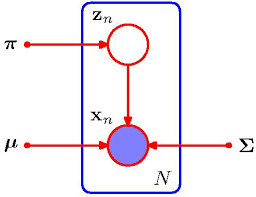
\includegraphics[scale=0.4]{./images/gmm.png}
	\end{center}
	\caption{Graphical representation of GMM model. The GMM models a joint distribution $p(\mathbf{x}, \mathbf{z})$ in terms of a marginal distribution $p(\mathbf{z})$ and conditional distribution $p(\mathbf{x}|\mathbf{z})$ to model $p(\mathbf{x})$. Each $\mathbf{x}_n$ is coupled with $\mathbf{z}_n$}
	\label{fig:gmm}
\end{figure}
Now we can work with the joint distribution $p(\mathbf{x,z})$ instead of the marginal distribution $p(\mathbf{x})$, which is hard to estimate directly as explained in \Cref{sec:intro_motivation}. 

Another quantity which plays a central role is the conditional proability of $\mathbf{z}$ given $\mathbf{x}$, $p(z_k=1|\mathbf{x})$. 
\begin{itemize}
\item $p(z_k=1) = \pi_k$ can be viewed as a prior of $z_k=1$
\item $\gamma(z_k)$: assignment probability or responsibility. This quantity will be updated through the Bayes Theorem.
\item[] $\rightarrow$  A simple explanation is that this is the classification result of $\mathbf{x}_n$.
\end{itemize}
\begin{align*}
\gamma(z_k) \equiv p(z_k=1|\mathbf{x}) & \equiv \frac{p(z_k=1)p(\mathbf{x}|z_k=1)}{\sum_{j=1}^{K}p(z_j=1)p(\mathbf{x}|z_j=1)} \\
& = \frac{\pi_k\mathcal{N}(\mathbf{x}|\boldsymbol{\mu}_k, \boldsymbol{\Sigma}_k)}{\sum_{j=1}^{K} \pi_j\mathcal{N}(\mathbf{x}|\boldsymbol{\mu}_j, \boldsymbol{\Sigma}_j)}
\end{align*}

\subsection{Maximum Likelihood}
Suppose we have a data set of observations $\mathbf{X}=\{\mathbf{x}_1,...,\mathbf{x}_n\}^{T}\in\mathbbm{R}^{N\times D}$ and we want to model the data distribution $p(\mathbf{X})$ using GMM. If we assume an \textrm{i.i.d.} data set, it can be expressed as follows: 
\begin{align*}
p(\mathbf{X}|\boldsymbol{\pi},\boldsymbol{\mu},\boldsymbol{\Sigma}) &=\prod_{n=1}^{N}\Bigg(\sum_{k=1}^{K}\pi_k\mathcal{N}(\mathbf{x}_n|\boldsymbol{\mu}_k, \boldsymbol{\Sigma}_k)\Bigg)\\
\end{align*}
then its loglikelihood function is given by:
\begin{align*}
\ln p(\mathbf{X}|\boldsymbol{\pi},\boldsymbol{\mu},\boldsymbol{\Sigma}) &= \sum_{n=1}^{N}\ln \Bigg(\sum_{k=1}^{K}\pi_k\mathcal{N}(\mathbf{x}_n|\boldsymbol{\mu}_k, \boldsymbol{\Sigma}_k)\Bigg)
\end{align*}

%In a single dimension case, 
%\begin{align*}
%	\ln p(x, \pi, \mu, \sigma) & =\sum_{n=1}^{N}\ln \sum_{k=1}^{K}\pi_k \frac{1}{\sigma_k \sqrt{2\pi_k}}\exp\Big(-\frac{1}{2}\Big(\frac{x_n-\mu_k}{\sigma_k}\Big)^2\Big)\\
%	\frac{\partial }{\partial \mu_k}\ln p(x, \pi, \mu, \sigma) & =\sum_{n=1}^{N} \frac{\pi_k \frac{1}{\sigma_k \sqrt{2\pi}}\exp\Big(-\frac{1}{2}\Big(\frac{x_n-\mu_k}{\sigma_k}\Big)^2\Big) \frac{x_n-\mu_k}{\sigma_k^2}}{\sum_{k=1}^{K}\pi_k \frac{1}{\sigma_k \sqrt{2\pi}}\exp\Big(-\frac{1}{2}\Big(\frac{x_n-\mu_k}{\sigma_k}\Big)^2\Big)}\\
%	& =\sum_{n=1}^{N} \underbrace{\frac{\pi_k \mathcal{N}(x_n|\mu_k, \sigma_k) }{\sum_{k=1}^{K}\pi_k \mathcal{N}(x_n|\mu_k, \sigma_k)}}_{=\gamma(z_{nk})}\frac{x_n-\mu_k}{\sigma_k^2}\\
%	\mu_k &=\frac{1}{N_k}\sum_{n=1}^{N} \gamma(z_{nk}) x_n,
%\end{align*}
%where 
%$N_k = \sum_{n=1}^{N} \gamma(z_{nk})$. $N_k$ can be interpreted as the effective number of points assigned to cluster $k$. 

Before, maximizing the likelihood, it is worth to emphasize two issues in GMM: (i) \textit{singularities} and (ii) \textit{identifiability}.

%\subsection{Singularity and Identifiability}
\paragraph{Singularity}
Suppose that one of the components of the mixture model, let us say the $j$-th component, has its mean $\mathbf{\mu}_j$ exactly equal to one of the data points so that $\mathbf{\mu}_j=\mathbf{x}_n$ for some value of $n$. This data point will then contributes a term in the likelihood function of the form 
$$\mathcal{N}(\mathbf{x}_n, \sigma_j^2\mathbf{I}) = \frac{1}{(2\pi)^{1/2}} \frac{1}{\sigma_j}$$
If we consider the limit $\sigma_j \to 0$, then we see that this term goes to infinity and so the log likelihood function will also go to infinity. Thus the maximization of the log likelihood function will also go to infinity. Thus the maximization of the log likelihood function is not a well posed problem because such sigularities will walways be present and will occur whenever one of the Gaussian components collapses onto a specific data point. 

\paragraph{Identifiability}
A further issue in finding MLE based solutions arises from the fact that for any given maximum likelihood solution, a $K$-component mixture will have a total ok $K!$ equivalent solutions corrsponding to the $K!$ ways of assigning $K$ sets of parameters to $K$ components. In other words, for any given point in the space of parameter values there will be a further $K!-1$ additional points all of which give rise to exactly the same distribution. 

\subsection{Expectation Maximization for GMM}

The goal of Expectation Maximization (EM) is to find maximum likelihood solutions for models having latent variables 
\begin{itemize}
	\item Suppose that it is hard to optimize $p(\mathbf{X}|\boldsymbol{\theta})$ directly.
	\item However, it is easier to optimize the complete-data likelihood function $p(\mathbf{X}, \mathbf{Z}|\boldsymbol{\theta})$ 
	\item In this case, we can use \textbf{EM algorithm}. EM algorithm is a general technique for finding maximum likelihood solutions for latent variable models. 
\end{itemize}

\begin{algorithm}
	Initialize the means $\boldsymbol{\mu}_k$, covariances $\boldsymbol{\Sigma}_k$ and mixing coefficients $\pi_k$ and evaluate the initial value of the log likelihood.\\
	\For{n}{
		E step: evaluate the responsibilities of $\mathbf{x}_n$ based on the current parameter values with the given parameters
		$$ \gamma(z_{nk})= p(z_k=1|\mathbf{x}_n) =  \frac{\pi_k\mathcal{N}(\mathbf{x}_n|\boldsymbol{\mu}_k, \boldsymbol{\Sigma}_k)}{\sum_{j=1}^{K} \pi_j\mathcal{N}(\mathbf{x}_n|\boldsymbol{\mu}_j, \boldsymbol{\Sigma}_j)}$$\\
		where $z_{nk}$ denote the $k$-th component of $\mathbf{z}_n$\\
		M step: maximize expectation
		\begin{itemize}
			\item $\boldsymbol{\mu}_k^{\textrm{new}} = \frac{1}{N_k}\sum_{n=1}^{N}\gamma(z_{nk})\mathbf{x}_n$
			\item $\boldsymbol{\Sigma}_k^{\textrm{new}} = \frac{1}{N_k}\sum_{n=1}^{N}\gamma(z_{nk})(\mathbf{x}_n-\boldsymbol{\mu}_k^{\textrm{new}})(\mathbf{x}_n-\boldsymbol{\mu}_k^{\textrm{new}})^T$
			\item $\pi_k^{\textrm{new}} = p(z_k=1) = \frac{N_k}{N}$
		\end{itemize}
	Evaluate the log likelihood to check for convergence of parameters
	$$\textrm{ln}p(\mathbf{X}|\boldsymbol{\pi},\boldsymbol{\mu},\boldsymbol{\Sigma}) = \sum_{n=1}^{N}\textrm{ln}\Bigg(\sum_{k=1}^{K}\pi_k\mathcal{N}(\mathbf{x}_n|\boldsymbol{\mu}_k, \boldsymbol{\Sigma}_k)\Bigg)$$
	}
	\caption{EM algorithm for GMM}
\end{algorithm}
	\begin{figure}[h]
	\begin{center}
		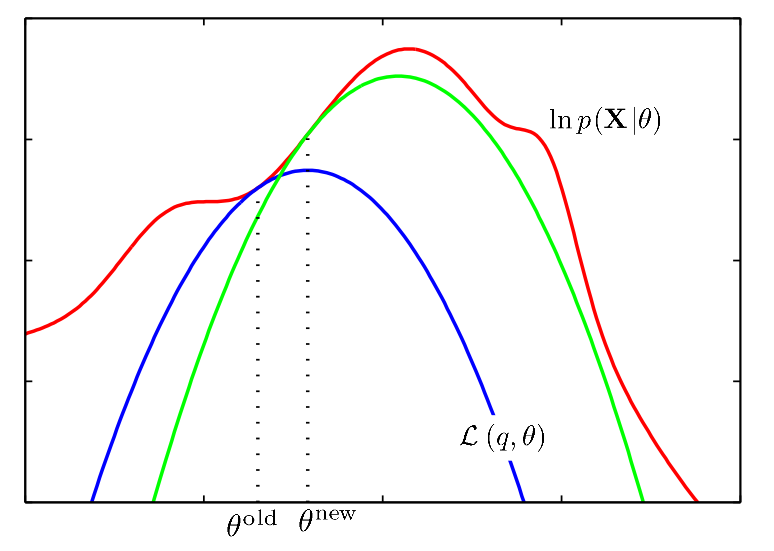
\includegraphics[scale=0.3]{./images/em_update.png}
	\end{center}
	\caption{M-step of EM algorithm}
	\label{fig:em2}
\end{figure}

%\section{KL Divergence}
%\begin{align*}
%	\textrm{KL}(q(x)||p(x)) = \int q(x)\log \frac{q(x)}{p(x)} = \mathbb{E}_q \Bigg[\log \frac{q(x)}{p(x)}\Bigg]
%\end{align*}

\section{Latent Variable Modeling}

For each object $x_i$, we establish additional latent variable $z_i$ which denotes the index of gaussian from which $i$-th object was generated. Then our model is
$$p(X,Z|\theta) = \prod_{i=1}^{n}p(x_i,z_i|\theta) = \prod_{i=1}^{n}p(x_i|z_i,\theta)p(z_i|\theta) = \prod_{i=1}^{n}\mathcal{N}(x_i|\mu_{z_i},\sigma_{z_i}^2)\pi_{z_i},$$
where $\pi_{j} = p(z_i=j)$ are prior probability of $j$-th gaussian and $\theta = \{\mu_j, \sigma_j, \pi_j\}_{j=1}^K$. If we know both $X$ and $Z$ then we can obtain explicit ML-solution:
$$\theta_{ML} = \argmax_{\theta}p(X,Z|\theta) = \argmax_{\theta}\log p(X,Z|\theta).$$
However, in practice, we don't know $Z$, but only know $X$. Thus, we need to maximize w.r.t. $\theta$ the log of incomplete likelihood
\begin{align}
	\log p(X|\theta) & = \int q(Z)\log p(X|\theta)dZ\\
	& = \int q(Z)\log \frac{p(X,Z|\theta)}{p(Z|X,\theta)}dZ\\
	& = \int q(Z)\log \frac{q(Z)p(X,Z|\theta)}{q(Z)p(Z|X,\theta)}dZ\\
	& = \int q(Z)\log \frac{p(X,Z|\theta)}{q(Z)}dZ+ \int q(Z)\log \frac{q(Z)}{p(Z|X,\theta)}dZ\\
	& = \underbrace{\int q(Z)\log \frac{p(X,Z|\theta)}{q(Z)}dZ}_{\textrm{ELBO, } \mathcal{L}(q,\theta)}+ \textrm{KL}(q(Z)||\log p(Z|X,\theta))
	\label{eq:elbo}
\end{align}
The first line uses that $Z$ is not related to $X$, so the integration does not affect $X$. Note that $p(X|\theta)$ in Eq.\ref{eq:elbo} (1) does not depend on $Z$. Also note that $p$ does not depend of $q$, \textbf{so maximizing ELBO is equal to minimizing the KL divergence}. 

By using ELBO, we are able to maximize the incomplete likelihood. If you see the KL term, it is trying to minimize the divergence between $q(Z)$ and $p(Z)$ through maximizing ELBO.

\subsection{ELBO}

Note that $\textrm{KL}(q(Z)||\log p(Z|X,\theta))\geq 0$, thus $\mathcal{L}(q,\theta) \leq \log p(X|\theta)$. In other words, $\mathcal{L}(q,\theta)$ is a \textbf{lower bound} on $\log p(X|\theta)$.

Let's see ELBO in a different perspective
\begin{align*}
	\mathcal{L}(q,\theta) &=  \int q(Z)\log \frac{p(X,Z|\theta)}{q(Z)}dZ\\
	&= \int q(Z)\Big[\log p(X,Z|\theta)- \log q(Z)\Big]dZ\\
	&= \int q(Z)\Big[\log p(Z|X,\theta)+\log p(X|\theta)-\log q(Z)\Big]dZ\\
	&= \int q(Z)\log p(X|\theta)dZ+\int q(Z) \log\frac{ p(Z|X,\theta)}{ q(Z)}dZ\\
	&= \log p(X|\theta)-\textrm{KL}(q(Z)|p(Z|X,\theta))
\end{align*}
To maximize the above equation, we need to minimize KL divergence. 

%\section{Variational Lower Bound}
%Function $g(\xi, x)$ is called variational lower bound for function $f(x)$ iff
%\begin{itemize}
%	\item For all $\xi$ for all $x$ if follows $f(x)\geq g(\xi, x)$
%	\item For any $x_0$ there exists $\xi(x_0)$ such that $f(x_0)=g(\xi(x_0), x_0)$
%\end{itemize} 

\subsection{Expectation Maximization}
We want to maximize ELBO, $\mathcal{L}(q,\theta)$, to minimize KL divergence between $q(Z)$ and $\log p(Z|X,\theta)$.
$$\max_{q,\theta}\mathcal{L}(q,\theta) = \max_{q,\theta}\int q(Z)\log \frac{p(X,Z|\theta)}{q(Z)}dZ.$$
We start from initial point $\theta_0$ and iteratively repeat \Ni E-step and \Nii M-step, iteratively:
\begin{itemize}
	\item E-Step: $\theta_0$ is fixed. 
		$$q(Z) = \argmax_{q}\mathcal{L}(q,\theta) = \argmin_{q}\textrm{KL}(q(Z)|p(Z|X,\theta)) = p(Z|X,\theta_0).$$ 
		\begin{itemize}
			\item This is because, maximizing ELBO is equal to minimizing KL divergence and the minimum $q$ can be achieved when $q$ is equal to $p(Z|X,\theta_0)$.
			\item Now, we just have to evaluate $p(Z|X,\theta_0)$.
		\end{itemize}
	\item M-Step: $q$ is fixed.
		$$\theta_* = \argmax_{\theta}\mathcal{L}(q,\theta) = \argmax_{\theta}\mathbb{E}_{q(Z)}[\log p(X,Z|\theta)]$$
		\begin{itemize}
			\item Can be accomplished by taking derivatives
			\item Set $\theta_0=\theta_*$ and go to the E-Step until convergence
		\end{itemize}
	
\end{itemize}

\subsection{Categorical Latent Variables}
$z_i \in \{1,...,K\}$
$$p(x_i|\theta) = \sum_{k=1}^{K}p(x_i|k,\theta)p(z_i=k|\theta)$$
is simply a finite mixture of distributions. 

E-Step:
$$q(z_i=k) = p(z_i=k|x_i,\theta) = \frac{p(x_k|z_i=k,\theta)p(z_i=k|\theta)}{\sum_{l=1}^{K}p(x_i|z_i=l,\theta)p(z_i=l|\theta)}$$
M-Step:
$$\argmax_{\theta}\mathbb{E}_{q(Z)}[\log p(X,Z|\theta)] = \sum_{i=1}^{n}\mathbb{E}_{q(z_i)}[\log p(x_i,z_i|\theta)] = \sum_{i=1}^{n}\sum_{k=1}^{K}q(z_i=k)\log p(x_i,k|\theta)$$

For GMM, we model $p(x|z)$ as Gaussian.

%\subsection{Continous Latent Variables}
%Continuous latent variables can be regarded as a mixture model of continous distributions. 
%$$p(x_i|\theta) = \int p(z_i|x_i,\theta) dz_i = \int p(x_i|z_i,\theta)p(z_i|\theta) dz_i$$
%E-step can be done in a closed from only in case of conjugate distributions, otherwise the true posterior is intractadble.
%$$q(z_i) = p(z_i|x_i,\theta) = \frac{p(x_k|z_i,\theta)p(z_i|\theta)}{\int p(x_i|z_i,\theta)p(z_i|\theta)dz_i}$$
%
%Typically, continuous latent variables are used for dimension reduction techniques also known as \textbf{representation learning.}

\chapter{Deep Generative Models}
\section{Variational Autoencoder}

Our goal is to find the data distribution $p(X)$. \Cref{fig:dgm} represents a general structure of deep generative model. As you can see, we first sample $z\sim p(z)$ and feed it into a deep neural network $f(z)$ and output $x$.

\begin{figure}[h]
	\begin{center}
		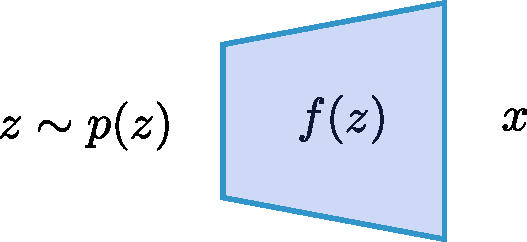
\includegraphics[scale=0.5]{./images/dgm.pdf}
	\end{center}
	\caption{General structure of deep generative models. This model does not infer $z$ from $x$.}
	\label{fig:dgm}
\end{figure}

VAE performs an inference by introducing a probabilistic encoder, called inference network. VAEs are generative model with a latent variable distributed according to some distribution $p(z_i)$. The observed variable is distributed according to a conditional distribution 
$$p_\theta(x_i|z_i)$$
This conditioning means the latent variable values are the one most likely given the observations. We also create a distribution $q_\phi(z_i|x_i)$. We would like to be able to encode our data into the latent variable space. Let's model the distribution.

\begin{itemize}
	\item $p_\theta(x_i|z_i)\sim \mathcal{N}(x_{i}|\mu(z_i), \sigma^2(z_i))$: A probabilistic decoder (or generative network, $\theta$)
	\item $q_\phi(z_i|x_i)$: A probabilistic encoder (or inference network $\phi$). We can choose a family of distributions for our conditional distribution $q$ (\eg standard Gaussian distribution). 
		$$q_\phi(z_i|x_i) = \mathcal{N}(z_i|\mu(x_i, W_1), \sigma^2(x_i, W_2)I),$$
	where $W_1$ and $W_2$ are network weights and collectively denoted as $\phi$. We create a neural network to model the distribution $q$ from our data in a non-linear manner. The outputs of the network are $\mu$ and $\sigma$. 
\end{itemize}

\begin{figure}[h]
	\begin{center}
		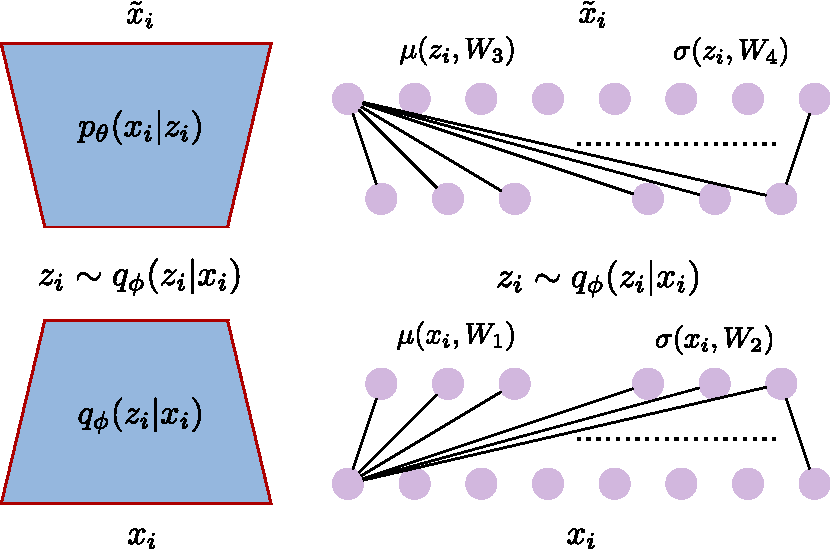
\includegraphics[scale=0.5]{./images/encoder.pdf}
	\end{center}
	\caption{Overview of variational autoencoder.}
	\label{fig:vae}
\end{figure}



\begin{align*}
	p(X,Z|\theta) &=  \prod_{i=1}^{n}\underbrace{p(x_i|z_i,\theta)}_{\textrm{Likelihood, Generator}}\underbrace{p(z_i|\theta)}_{\textrm{Prior on latent variable}}\\
	&= \prod_{i=1}^{n} \mathcal{N}(x_{i}|\underbrace{\mu(z_i), \sigma^2(z_i)}_{\textrm{Non-linear}}) \mathcal{N}(z_i|0, I)
\end{align*}

Subsequently, marginal distributions can be expressed as follows under i.i.d. assumption:
\begin{align*}
	p(X|\theta) &= \prod_{i=1}^{n} p(x_i|\theta) \\
	&= \prod_{i=1}^{n} \int p(x_i, z_j|\theta) dz_j \\
	& = \prod_{i=1}^{n} \int p(x_i|z_i, \theta)p(z_i|\theta)dz_i \\
	& = \prod_{i=1}^{n} \int \mathcal{N}(x_{i}|\mu(z_i), \sigma^2(z_i)) \underbrace{\mathcal{N}(z_i|0, I)}_{\textrm{Mixture weight}} dz_i
\end{align*}

\begin{itemize}
	\item As you can see, the marginal distribution $p(X|\theta)$ becomes a mixture of Gaussian (infinite mixture of Gaussian). 
	\item Even though $p(x|z)$ and $p(z)$ are normal, $p(x)$ is not normal, because it is a mixture distribution.
	\item The non-linearity of Gaussian parameters (modeled by a neural network), conjugacy between the prior and the likelihood does not hold anymore.
%	\item Diagonal covariance matrix does not mean the independence between elements of $x$.
	\item Again, $\mu$ and $\sigma$ is non-linear function of $z$ modeled by some non-linear neural network. The neural network works as a powerful non-linear parameter approximator (based on universal approximation theorem). 
	\item Simple prior is used. Let's consider the data $x$ is an image of $100\times 100$ pixels. Then the covariance matrix has to be $10000\times 10000$. Thus, it is common to set a simple prior such as the standard Gaussian (covariance matrix is diagonal matrix). However, even if we set a simple distribution, with the infinite mixture of Gaussian, we can model any distribution.
	\item VAE uses a global parametric model to predict the local
		variational parameters for each data point (amortized inference). 
%	\item Under the simple standard Gaussian prior assumption, the generator, $p(x_i|z_i,\theta)$, returns factorized Gaussian whose mean and variance are non-linear functions of latent variable modelled by deep neural network parameterized by $\theta$.
%	$$p(x_i|z_i,\theta) = \mathcal{N}(x_{i}|\mu(z_i), \sigma^2(z_i))$$
%	\item VAEs uses a simple prior over latent variables and complicated and powerful generator (neural network).
	\item It allows to convert complicated large-dimensional data distributions into simple lower-dimensional latent variable representations.  
%	\item $Std = e^{\frac{1}{2}\log (Var)}$, thus output is the log var
\end{itemize}

Then, we can train VAE using variational inference with ELBO:

$$\mathcal{L}(\phi,\theta) = \mathbbm{E}_{q_{\phi}(z|x)}[\log p_{\theta}(x|z)] - D_{\textrm{KL}}(q_{\phi}(z|x)||p_{\theta}(z))$$

\begin{itemize}
	\item The first term can be estimated by using
		$$\mathbbm{E}_{q_{\phi}(z|x)}[\log p_{\theta}(x|z)]\approx \frac{1}{N}\sum_j \log p_{\theta}(x_i|z_j).$$
	\item The second term can be solve analytically for some distributions like Gaussian.
	\item For training, we need to use a reparameterization trick. 
\end{itemize}




%\footnotetext[1]{Uncorrelated relationship does not imply the independence (independence makes covariance to be diagonal). If two variables are uncorrelated, $Cov(x_i,x_j)=0 $, there is no linear relationship between them.}
%\footnotetext[2]{In practice, simple prior could be a problem.}


\backmatter
% bibliography, glossary and index would go here.

\nocite{*}
\bibliographystyle{unsrt}
\bibliography{references}
\end{document}
